\documentclass[tikz,border=12pt]{standalone}
\usepackage[american]{circuitikz}
% Shared visual language for standalone EMT block diagrams.
\usepackage{amsmath}
\usetikzlibrary{arrows.meta,backgrounds,calc,fit,positioning}

\tikzset{
    emt diagram/.style = {>={Stealth[length=2.4mm]}},
    line/.style        = {semithick, rounded corners=6pt},
    block/.style       = {draw, semithick, fill=white,
                          minimum height=1cm, minimum width=2.3cm},
    hblock/.style      = {block, minimum width=2.24cm, minimum height=1.3cm},
    vblock/.style      = {block, minimum width=1.3cm, minimum height=2.24cm},
    sum/.style         = {draw, semithick, fill=white, circle,
                          inner sep=2.6pt},
    signal/.style      = {circle, fill, inner sep=1.4pt,
                          label distance=3pt},
    sig/.style         = {font=\small},
    pm/.style          = {font=\scriptsize},
    wire jump/.style   = {line,
                          preaction={draw=white, line width=3pt,
                                     line cap=round}},
    enclosure/.style   = {draw, dashed, semithick, rounded corners=4pt},
    operator enclosure/.style = {enclosure, inner xsep=7mm, inner ysep=6mm}
}


\tikzset{
    igbt/.style = {nigbt, bodydiode, semithick, scale=1.2}
}

\begin{document}
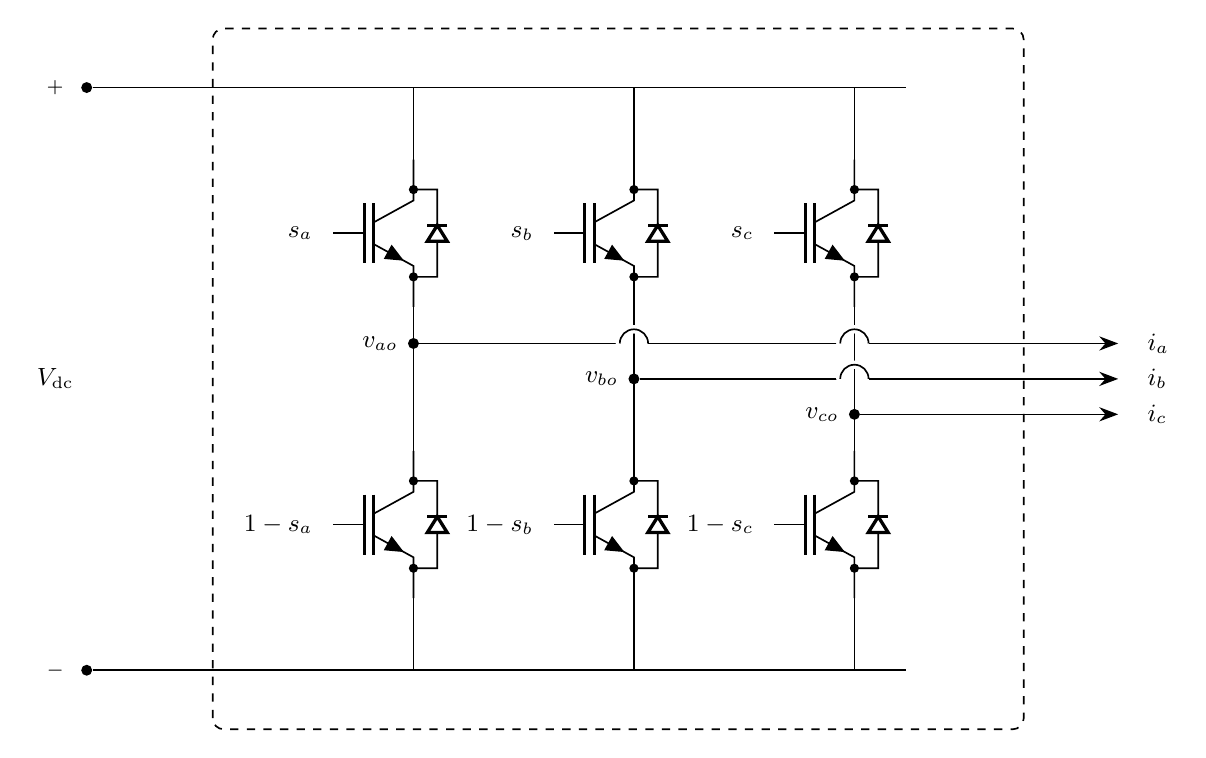
\begin{tikzpicture}[emt diagram]

% ================= DC input =================
\node[signal] (dc+) at (-6.95, 3.7) {};
\node[signal] (dc-) at (-6.95, -3.7) {};
\draw[line] (dc+) -- (3.45, 3.7);
\draw[line] (dc-) -- (3.45, -3.7);

\node[pm] at (-7.35, 3.7) {$+$};
\node[sig] at (-7.35, 0) {$V_{\mathrm{dc}}$};
\node[pm] at (-7.35, -3.7) {$-$};

% ================= Phase-a IGBTs =================
\node[igbt] (Sa+) at (-2.8, 1.85) {};
\node[igbt] (Sa-) at (-2.8, -1.85) {};
\draw[line] (Sa+.C) -- (-2.8, 3.7);
\draw[line] (Sa+.E) -- (-2.8, 0);
\draw[line] (Sa-.C) -- (-2.8, 0);
\draw[line] (Sa-.E) -- (-2.8, -3.7);
\node[sig, anchor=east] at ($(Sa+.G)+(-0.15,0)$) {$s_a$};
\node[sig, anchor=east] at ($(Sa-.G)+(-0.15,0)$) {$1-s_a$};

% ================= Phase-b IGBTs =================
\node[igbt] (Sb+) at (0, 1.85) {};
\node[igbt] (Sb-) at (0, -1.85) {};
\draw[line] (Sb+.C) -- (0, 3.7);
\draw[line] (Sb+.E) -- (0, 0);
\draw[line] (Sb-.C) -- (0, 0);
\draw[line] (Sb-.E) -- (0, -3.7);
\node[sig, anchor=east] at ($(Sb+.G)+(-0.15,0)$) {$s_b$};
\node[sig, anchor=east] at ($(Sb-.G)+(-0.15,0)$) {$1-s_b$};

% ================= Phase-c IGBTs =================
\node[igbt] (Sc+) at (2.8, 1.85) {};
\node[igbt] (Sc-) at (2.8, -1.85) {};
\draw[line] (Sc+.C) -- (2.8, 3.7);
\draw[line] (Sc+.E) -- (2.8, 0);
\draw[line] (Sc-.C) -- (2.8, 0);
\draw[line] (Sc-.E) -- (2.8, -3.7);
\node[sig, anchor=east] at ($(Sc+.G)+(-0.15,0)$) {$s_c$};
\node[sig, anchor=east] at ($(Sc-.G)+(-0.15,0)$) {$1-s_c$};

% ================= Phase terminals =================
\node[signal, label={[sig]left:$v_{ao}$}] (a) at (-2.8, 0.45) {};
\node[signal, label={[sig]left:$v_{bo}$}] (b) at (0, 0) {};
\node[signal, label={[sig]left:$v_{co}$}] (c) at (2.8, -0.45) {};

\draw[line] (a) -- (-0.18, 0.45);
\draw[wire jump] (-0.18, 0.45)
    arc[start angle=180, end angle=0, radius=0.18];
\draw[line] (0.18, 0.45) -- (2.62, 0.45);
\draw[wire jump] (2.62, 0.45)
    arc[start angle=180, end angle=0, radius=0.18];
\draw[->, line] (2.98, 0.45) -- (6.15, 0.45);

\draw[line] (b) -- (2.62, 0);
\draw[wire jump] (2.62, 0)
    arc[start angle=180, end angle=0, radius=0.18];
\draw[->, line] (2.98, 0) -- (6.15, 0);

\draw[->, line] (c) -- (6.15, -0.45);

\node[sig, anchor=west] at (6.40, 0.45) {$i_a$};
\node[sig, anchor=west] at (6.40, 0) {$i_b$};
\node[sig, anchor=west] at (6.40, -0.45) {$i_c$};

% ================= Model enclosure =================
\draw[enclosure] (-5.35, -4.45) rectangle (4.95, 4.45);

\end{tikzpicture}
\end{document}
